\section{Data Processing and Other Instructions}

\subsection{Arithmetic Operations}
\nonumsidenote{There are six basic arithmetic operations:
\begin{tabular}{ll}
	\texttt{add} & Addition \\
	\texttt{adc} & Addition with Carry \\
	\texttt{sub} & Subtract \\
	\texttt{suc} & Subtraction with Carry \\
	\texttt{neg} & Negate \\
	\texttt{ngc} & Negate with Carry \\
\end{tabular}}
\begin{lstlisting}
#include <stdio.h>
static int x = 5;
static int y = 8;
int main(void) {
	int sum;
	sum = x + y;
	printf("The sum is %d\n",sum);
	return 0;
}
\end{lstlisting}
\nonumsidenote{\begin{itemize}[leftmargin=*]
	\item \textbf{Data Segment}:
	\item[*] \texttt{fmt} holds \texttt{"The sum is \%d\textbackslash n\textbackslash0"}.
	\item[*] \texttt{x} contains the integer \texttt{5}.
	\item[*] \texttt{y} contains the integer \texttt{8}.
	\item \textbf{Stack Frame during main Execution}:
	\item[*] Temporary space for \texttt{x29} and \texttt{x30}.
	\item[*] Stack pointer adjusts as needed for the function call and return.
\end{itemize}}
\begin{lstlisting}
		.data
fmt:	.asciz	"The sum is %d\n"
		.algin	2
x:		.word 	5
y:		.word 	8
		.text
		.type 	main, %function
		.global	main
main:
		stp 	x29, x30, [sp, #-16]! 	// Push FP, LR onto the stack
		//	sum = x + y
		adr 	x14, x					// Calculate address of x
		adr 	x15, y					// Calculate address of y 
		ldr 	x4, [x14] 				// Load x
		ldr 	x5, [x15] 				// Load y
		add 	x1, x4, x5 				// x1 = x4 + x5
		
		//  printf("The sum is %d\n", sum)
		adr 	x0, fmt 				// Calculate address of fmt
		bl 	printf 				// Call the printf function
		
		// return 0
		mov 	w0, #0
		ldp 	x29, x30, [sp], #16 	// Pop FP and LR from the stack
		ret 								// Return from main
		.size 	main,(. - main)
\end{lstlisting}

%\begin{table}[h!]
%%\caption*{Data Section (\texttt{.data})}
%\begin{tabular}{ll}\toprule[1.2pt]
%	\texttt{.data} & This section holds initialized data accessed\\
%	&  or referenced by the program. \\ \hline
%	\texttt{fmt: .asciz "The sum is \%d\textbackslash n"} & Declares a null-terminated string \texttt{fmt} for \texttt{printf}. \\
%	& The \texttt{\%d} is a placeholder for an integer, \\
%	& and \texttt{\textbackslash n} is a newline character.\\ \hline
%	\texttt{.align 2} & Aligns the following data to \\
%	& a 2-byte boundary for optimal memory access. \\ \hline
%	\texttt{x: .word 5} & Declares a 32-bit integer variable \texttt{x} initialized to the value \texttt{5}.\\ \hline
%	\texttt{y: .word 8} & Declares a 32-bit integer variable \texttt{y} initialized to the value \texttt{8}. \\ \bottomrule[1.2pt]
%\end{tabular}
%\end{table}
%
%\begin{table}[h!]\setstretch{1}
%%\caption*{Text Section (\texttt{.text})}
%\begin{tabular}{ll}\toprule[1.2pt]
%	\texttt{.text} & Indicates the start of the code section. \\ \hline
%	\texttt{.type main, \%function} & Specifies that \texttt{main} is a function. \\ \hline
%	\texttt{.global main} & Declares \texttt{main} as a global symbol. \\ \hline
%	\texttt{.extern printf} & Declares \texttt{printf} as an external function. \\ \bottomrule[1.2pt]
%\end{tabular}
%\end{table}
%
%\begin{table}[h!]\setstretch{1}
%%\caption*{Text Section (\texttt{.text})}
%\begin{tabular}{ll}\toprule[1.2pt]
%	\texttt{stp x29, x30, [sp, \#-16]!} & Pushes the current frame pointer \texttt{x29} \\
%	& and link register \texttt{x30} onto the stack. \\ \hline
%	\texttt{mov x29, sp} & Sets \texttt{x29} as the frame pointer \\
%	& for easier reference within the function. \\ \bottomrule[1.2pt]
%\end{tabular}
%\end{table}
%
%\begin{table}[h!]\setstretch{1}
%%\caption*{Text Section (\texttt{.text})}
%\begin{tabular}{ll}\toprule[1.2pt]
%	\texttt{adr x14, x} & Loads the address of \texttt{x} into register \texttt{x14}. \\
%	\texttt{adr x15, y} & Loads the address of \texttt{y} into register \texttt{x15}. \\
%	\texttt{ldr x4, [x14]} & Loads the 32-bit value at address \texttt{x14} (address of \texttt{x}) into register \texttt{x4}. \\
%	\texttt{ldr x5, [x15]} & Loads the 32-bit value at address \texttt{x15} (address of \texttt{y}) into register \texttt{x5}. \\
%	\texttt{add x1, x4, x5} & Adds \texttt{x4} and \texttt{x5} and stores the result in \texttt{x1}. \\ \bottomrule[1.2pt]
%\end{tabular}
%\end{table}
%
%\begin{table}[h!]\setstretch{1}
%%\caption*{Text Section (\texttt{.text})}
%\begin{tabular}{ll}\toprule[1.2pt]
%	\texttt{adr x0, fmt} & Loads the address of the format string \texttt{fmt} into register \texttt{x0}. \\
%	\texttt{bl printf} & Calls \texttt{printf}, passing \texttt{fmt} (in \texttt{x0}) and the sum (in \texttt{x1}). \\ \bottomrule[1.2pt]
%\end{tabular}
%\end{table}
%
%\begin{table}[h!]\setstretch{1}
%%\caption*{Text Section (\texttt{.text})}
%\begin{tabular}{ll}\toprule[1.2pt]
%	\texttt{mov w0, \#0} & Sets the return value of \texttt{main} to \texttt{0}. \\
%	\texttt{ldp x29, x30, [sp], \#16} & Restores \texttt{x29} and \texttt{x30} from the stack. \\
%	\texttt{ret} & Returns from the \texttt{main} function. \\ 
%	\texttt{.size main, (. - main)} & Calculates the size of the \texttt{main} function \\
%	& by subtracting the address of \texttt{main} from the current address. \\ \bottomrule[1.2pt]
%\end{tabular}
%\end{table}

\begin{figure}[h!]\centering
	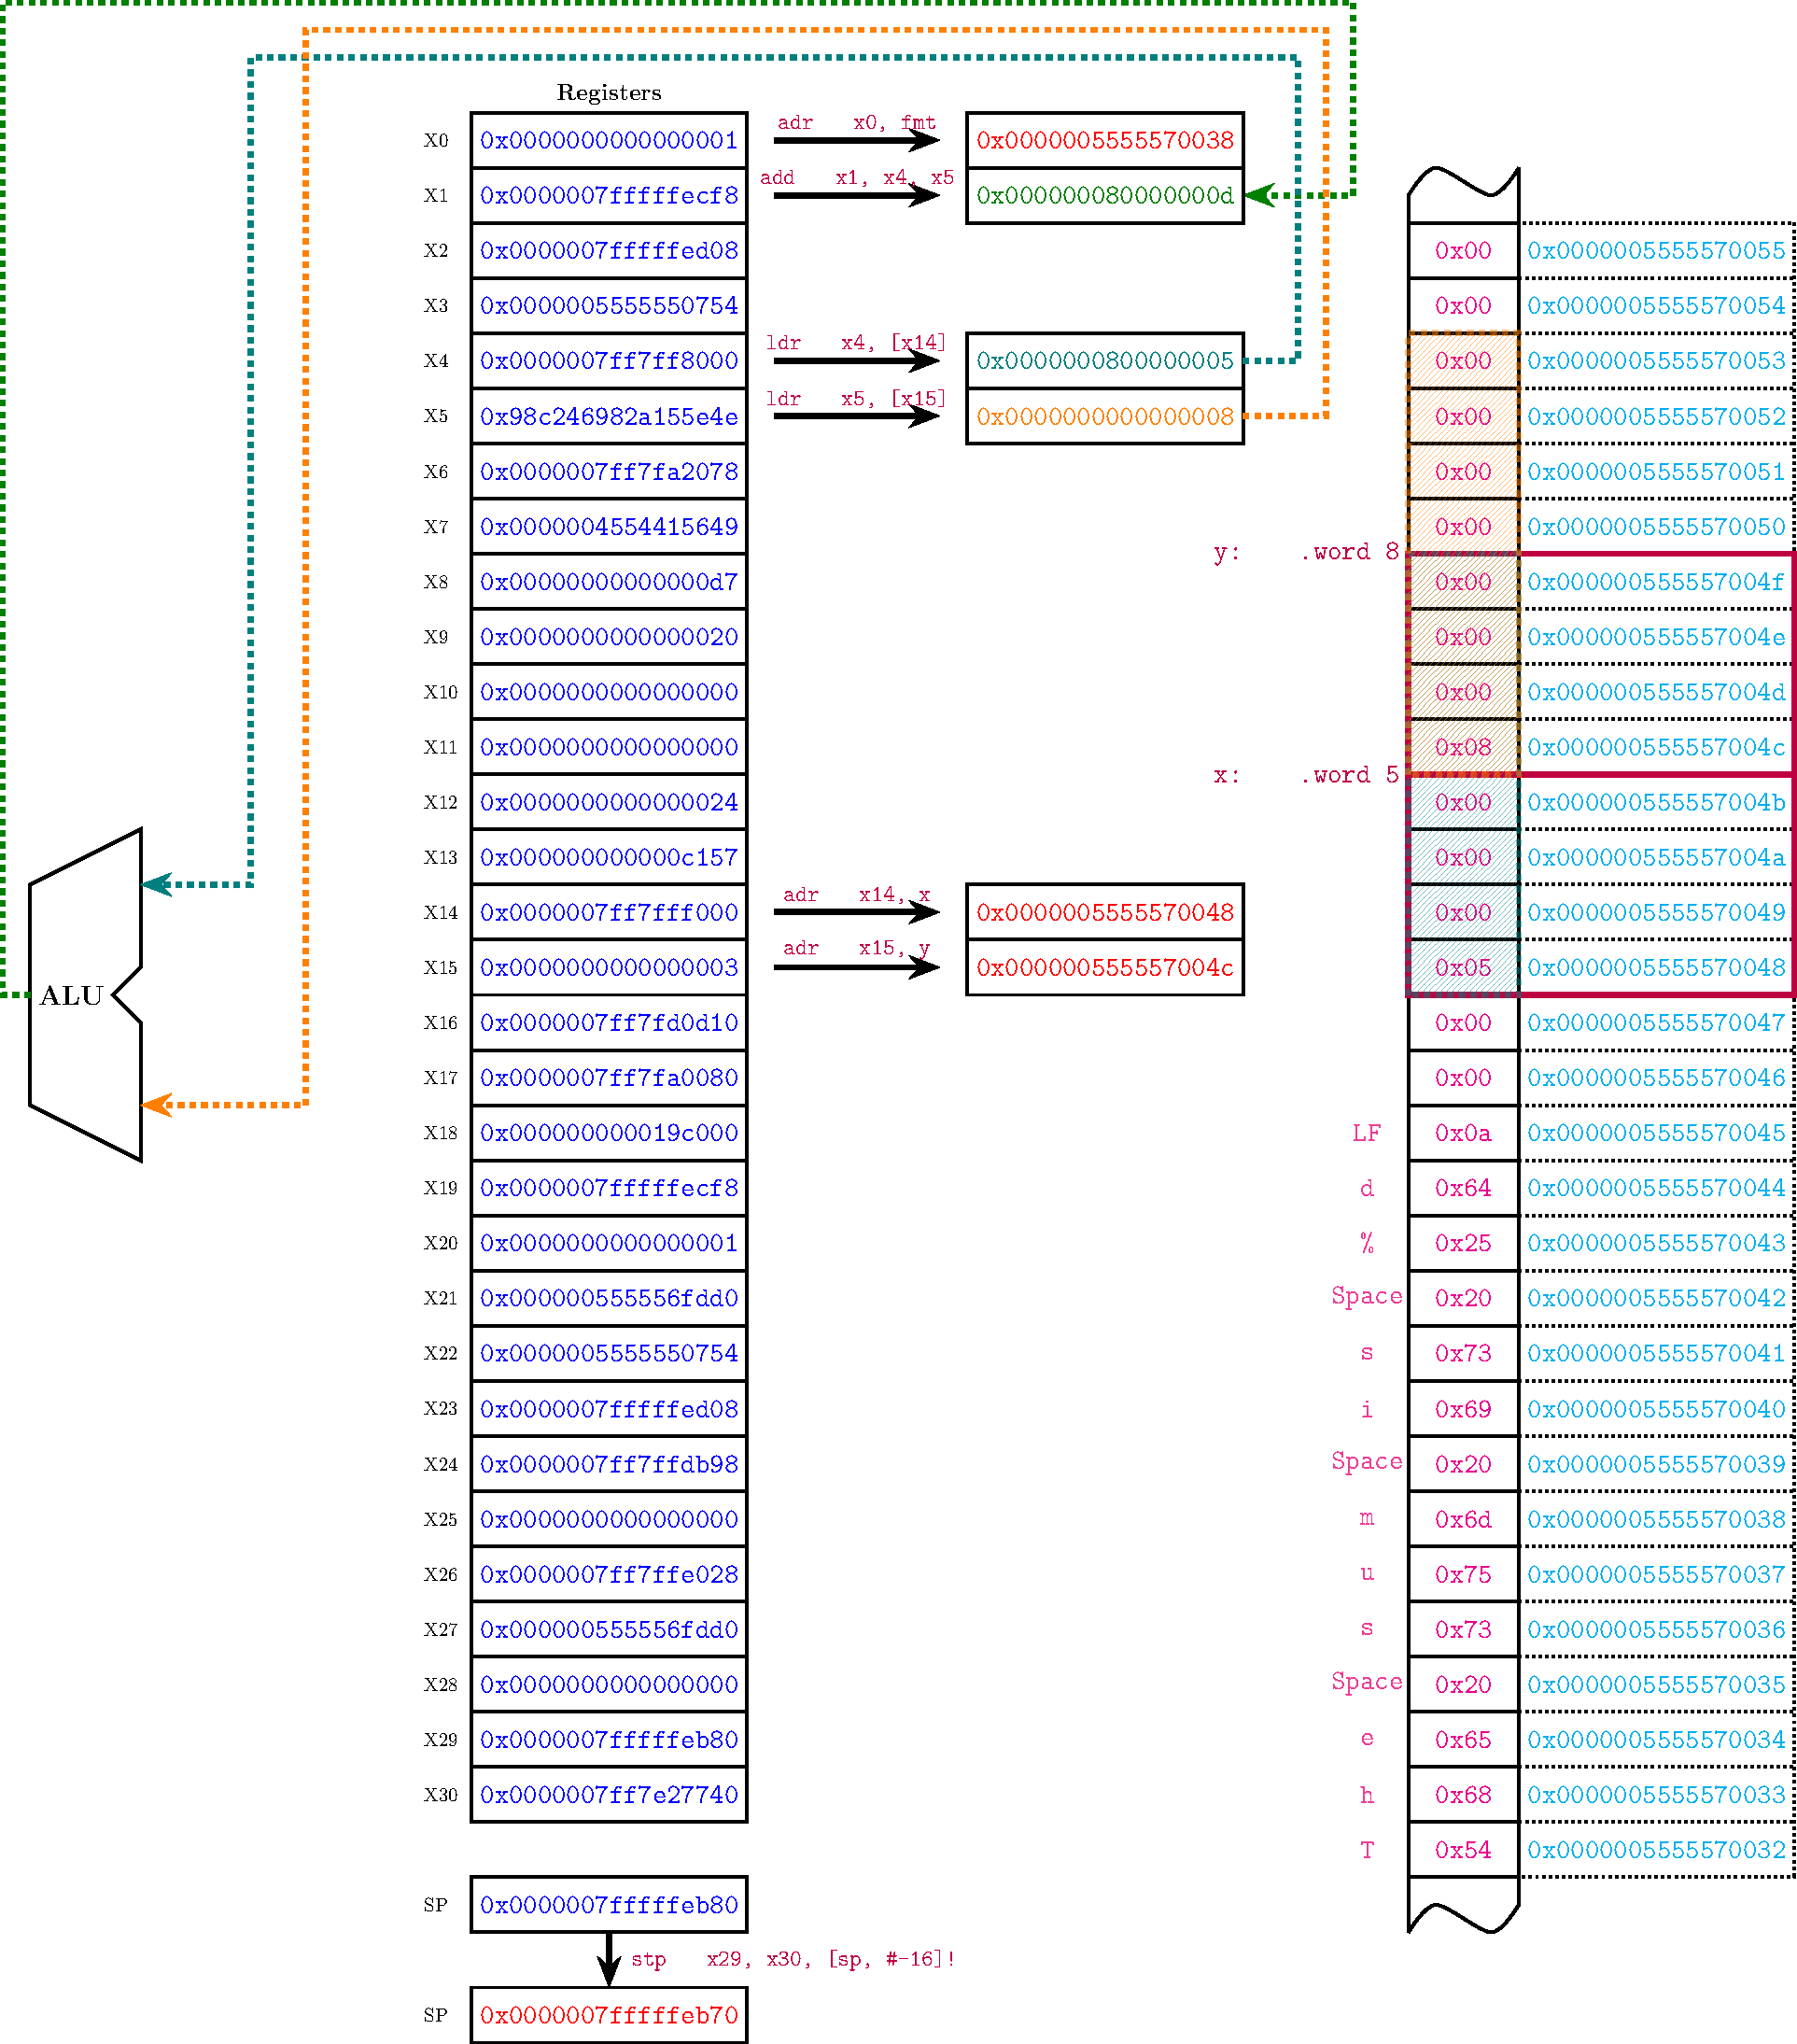
\includegraphics[width=1.5\textwidth]{architectures/sum.pdf}
\end{figure}

\newpage
\subsection{Shift Operations}
\subsection{Multiply Operations with Overflow}
\subsection{Multiply Operations with 64-bit results}
\subsection{Multiply Operations with 128-bit results}
\subsection{Division Operations}
\subsection{Comparison Operations}
\subsection{Conditional Operations}

